The context diagram in Figure~\ref{fig:TrigProcContext} shows the different interfaces to the NSW Trigger Processor
and the signal flow through the trigger system.
The NSW Trigger Processor is implemented in FPGAs on mezzanine cards of an ATCA carrier card.
One NSW sector (16~per end-cap wheel) is implemented on one FPGA (Xilinx Virtex~7 XC7VX690T).
Input and output fibers connect directly to the mezzanine cards.
Some services are on the carrier card which has an Ethernet connection.
The plan for the fiber connections from the front ends to the readout and trigger processors in USA-15 is shown in Appendix~\ref{app:specs-fibers}.

\begin{figure}[h]
	\centering
	%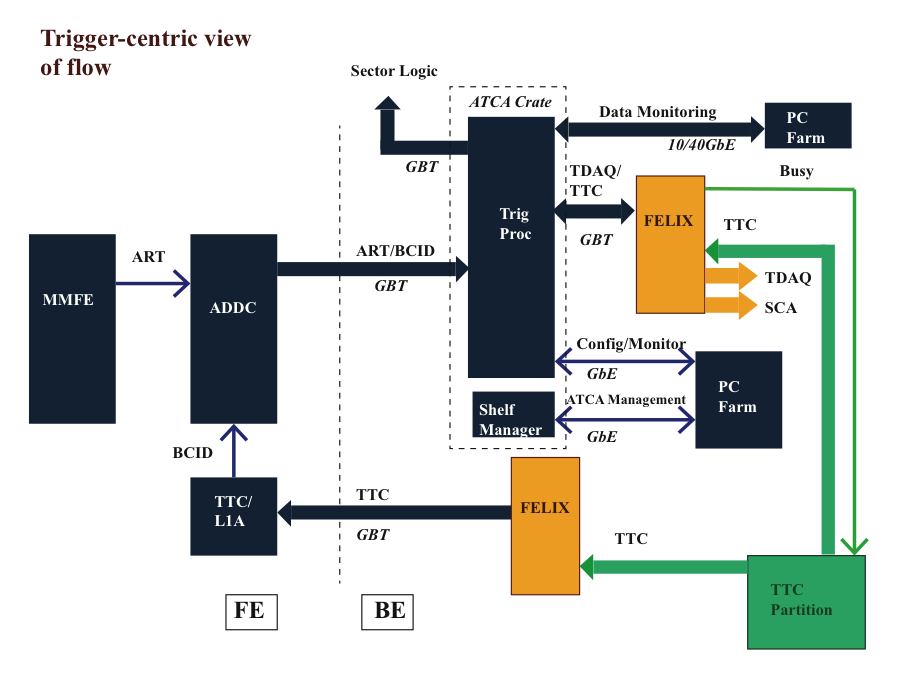
\includegraphics[width=0.8\textwidth]{specs/MMTriggerProcessorConfiguration}
	%\caption{Configuration relevant to the MM Trigger Processor.}
	%\label{fig:MMTriggerConfiguration}
	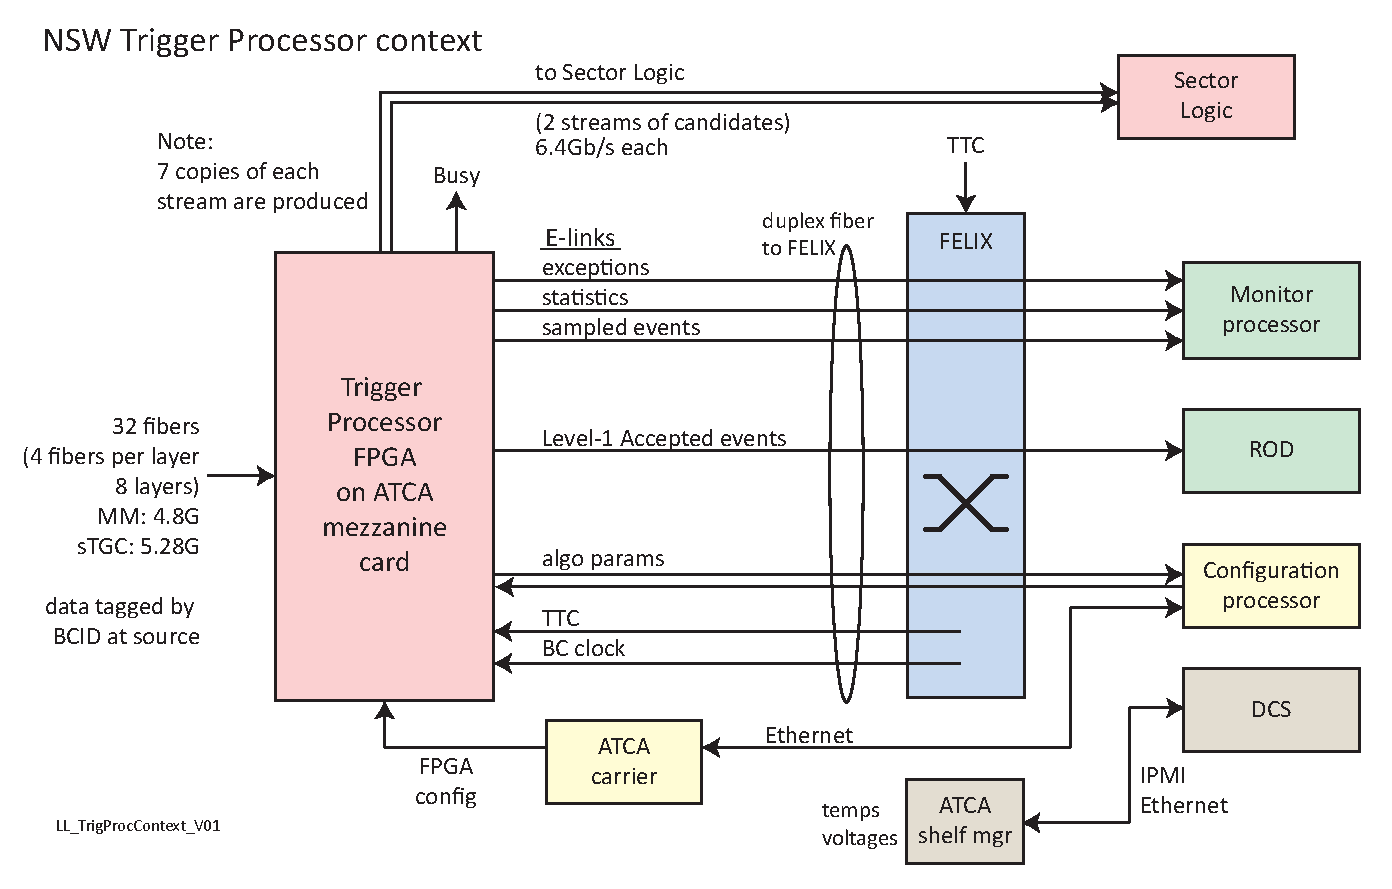
\includegraphics[width=0.97\textwidth]{figures/LL_TrigProcContext_V01.pdf}
	\caption{Trigger Processor context diagram}
	\label{fig:TrigProcContext}
\end{figure}

\vspace{-15pt}
\paragraph{Mezzanine card connections}
\begin{itemize}\itemsep-4pt\vspace{-5pt}
\item 32 input fibers from ADDC (MM) or Router (sTGC)
\item Several output fibers to the Sector Logic
\item An output fiber to FELIX which carries the following data flows on different E-links:
    \begin{itemize}\itemsep-6pt\vspace{-4pt}
    \item Level-1 Accept event readout
    \item Exception messages
    \item Statistics
    \item Sampled events
    \item Algorithm parameters
    \item TTC and BC clock
    \end{itemize}
\end{itemize}

\vspace{-15pt}
\paragraph{Services via the ATCA carrier}
\begin{itemize}\itemsep-4pt\vspace{-5pt}
\item Configuration of the FPGA itself via Ethernet
\item Temperature and voltage monitoring to DCS via Shelf Manager Ethernet
\end{itemize}

%Should the Trigger Processor FPGA become excessively utilized for the trigger algorithms,
%it is possible to move some of the non-algorithm logic to the FPGA on the carrier board.


\subsection{Trigger Processor Latency}
\label{sec:latency}

The trigger signal delivery time to the MuCTPI has to happen within 57~Bunch Crossings (BCs) (an increase of 3.5~BCs from the \PhaseZero system).
The New Sector Logic requires 16~BCs from the time it receives the trigger signal from the NSW and BW until it delivers it to the MuCTPI (5 BCs for serializer/deserializer,
9~BCs for trigger processing, and 2~BCs for transmission via fiber).
This leaves 43~BCs (1075~ns) for the full NSW trigger processing chain (including 2~BCs to merge the MM and sTGC trigger streams and time for the signal transmission to the Sector Logic).

The latency of the current design of the NSW trigger chain is at the
boundary of the required value, leaving no contingency.
It is therefore imperative to keep the latency as low as possible at
every step of the chain, including at the Trigger Processor.
The TP latency estimation is given in Table\,\ref{tab:latency} for both chamber technologies.
The accounting includes the input/output serializers, the trigger algorithm, the transmission time to the Sector Logic,
and the algorithm that merges the \MM and \stgc streams. The merging is currently planned to occur in the \stgc FPGA.

\begin{table}[htbp]
\centering
\begin{tabular}{l|cc|cc|l}
%\hline\hline
%\toprule
\toprule
    &\multicolumn{2}{c|}{sTGC} & \multicolumn{2}{c|}{MM} & \\
                                    & min   & max   & min  & max    &  Notes           \\
                                    & (ns)  & (ns)  & (ns) & (ns)   &                  \\
\midrule
Input deserializer (Rx)             & 40    & 40    & 44    & 44    &   \\
Trigger algorithm                   & 56    & 56    & 56    & 56    & 320\,MHz clock  \\
Stream merging algorithm            & 25    & 50    & --    & --    & Assigned to sTGC \\
Re-synch to 320 MHz clock           & 0     & 3.1   & 0     & 3.1   & $45^{\circ}$ phase chosen to  \\
\ \ driving output serializer       &       &       &       &       & \ \ \ best match pipeline length \\
Output to Sector Logic              & 25    & 30    & 25    & 30    & Deserializer on Sector Logic \\
\ \ serializer (Tx only)            &       &       &       &       & \ \ \ latency budget  \\
Fiber to Sector Logic               & 20    & 25    & 20    & 25    & 4-5\,m fiber @ 5\,ns/m  \\
\midrule
Total                               & 166   & 204.1 & 145   & 158.1 &     \\
\bottomrule
%\bottomrule
\end{tabular}
\caption{Trigger Processor latency for the \MM and \stgc streams. The
  time required to merge the two streams is assigned only to the
  \stgc, since the merging would occur in the sTGC FPGA. 
\label{tab:latency}  }
\end{table}

% Deserializer comment: GBT-FPGA (optimized) - includes GTX-TX  (Kai Chen)
